\section{Results and Discussion}
\label{sec:results}

\cmtDK[inline]{15 pages}
\subsection{Pre-experiments without language games}
\subsubsection{Coordinate predictor}
%     \item visualizations of predictions
%     \item difference between layers of feature extractors (especially compare to baseline learned from scratch)
%     \item masking is helping very much (especially for Dale-2)
%     \item visualizations show that model only focuses on center of the image


\begin{figure}[h]
    \centering
    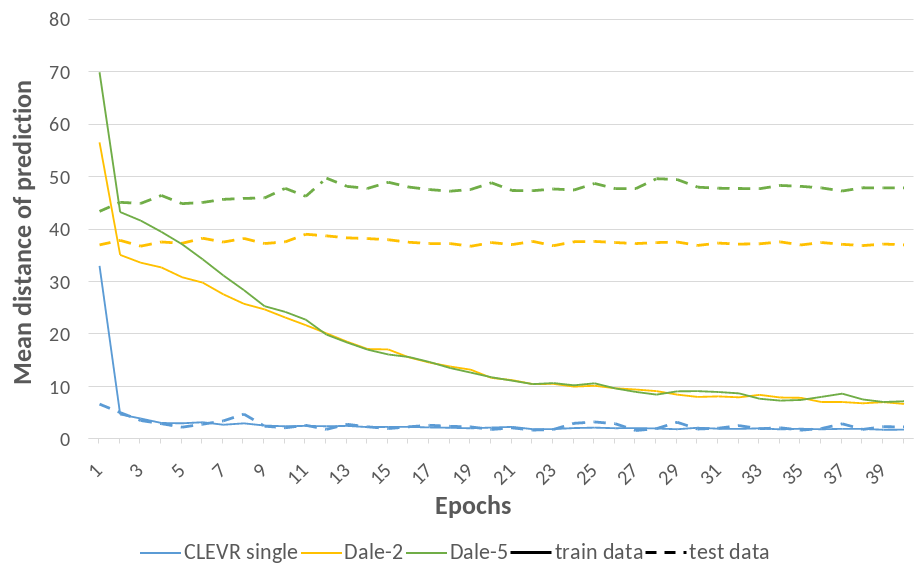
\includegraphics[width=0.8\linewidth]{figures/coordinate-predictor_loss.png}
    \caption{Mean distance between predicted coordinates and ground truth in pixels on different datasets}
    \label{fig:coordinate-predictor_loss}
\end{figure}

Figure \ref{fig:coordinate-predictor_loss} shows the results of the coordinate predictor that doesn't include any information about the target object.
The used feature extractor for these results is \emph{Resnet-3}, but the results don't differ significantly with other feature extractors.
As can be seen, the success between the different datasets differ significantly.
The more objects are present in an image, the worse the model performs.
The model converges for the CLEVR single dataset after around 20 epochs to a mean distance of around 2 pixels.
This prediction even though not perfectly on the center point is always on the object.
Opposed to that, using the Dale-2 dataset with two objects, the mean distance is from the first epoch between 37 and 38 pixels.
With five objects in the Dale-5 dataset, the model only predicts a mean distance of around 45 pixels in the beginning, which worsens with a rising number of epochs to 48 pixels.

An interesting observation is the difference of the mean distances between training and testing data.
The training distance is constantly approaching zero, while the testing loss is staying constant or even getting higher.
This points to the fact that the model is not generalizing the task and learning abstract patterns that can be applied to unseen data, but instead learning the training data by heart.
That is especially visible for the Dale-5 dataset, where learning the patterns of the training data looses even the ability to interpret some patterns in the testing data.
Applying a higher dropout didn't have an impact on the results.

This behavior is indeed not very surprising.
First, these results show that the model is able to derive geometrical information from abstract feature, extracted by a feature extractor.
Geometrical information therefore doesn't get lost during this abstraction, but the model is able to point to a specific object, as long as only one object is part of the image.
Secondly, more than one objects present in an image confuse the model, and it is not able to consistently point to one of them.
This can have multiple reasons, for instance that models lacks the ability to separate objects in the extracted features.
But even given, the model is able to do that and could determine the location of each object in the scene given the feature, it would not be able to tell, which of these is the actual target object.
The guess is then more or less random.
This especially applies to the Dale-2 dataset, where an identification of the target object just based on one distractor is impossible; both of the present objects are unique.
For the Dale-5 dataset, the model could in theory learn that the target object is always the one object which is unique in respect to its and the distractors' attributes.
This task on the other hand seems very difficult to learn.
In conclusion, the models are able to predict geometrical coordinates, but need more information about the target object to identify it.

When the target object \textbf{attributes are encoded as one-hot vectors} and added to the input, the results don't improve.
One factor that now has a much higher impact is the feature extractor that is used.
Table \ref{tab:feature-extractor-mean-distances} compares the mean distances the models predict for the different feature extractors.
The results are shown for the models trained on the Dale-2 and Dale-5 datasets for training and test data.
First, a big difference can be seen between the datasets.
The model doesn't converge on the correct coordinates for the Dale-5 dataset at all, looking at the test data.
All resulting mean distances are in a similar range around 50 pixels.
Using the Dale-2 dataset, the behavior is a little different.
All ResNet extractors with four residual blocks and optionally additional average pooling and classifier layers reach similar scores as the experiments before without any one-hot encodings.
Interestingly, using less residual layers, the model doesn't converge at all and the mean distances jump up and down between the epochs.
This effect also applies when using less residual blocks.
Using the VGG, both using VGG-avg and VGG-cls2 achieve a similar performance, while the others predict coordinates between 43 and 46 pixels away.
\cmtDK{compare to scratch}

\begin{table}[h]
    \centering
    \begin{tabular}{rcccc}
        \toprule
                            & \multicolumn{2}{c}{\textbf{Dale-2}} & \multicolumn{2}{c}{\textbf{Dale-5}}                                   \\\cmidrule(lr){2-3}\cmidrule(lr){4-5}
                            & train                               & test                                & train          & test           \\\midrule
        \textbf{VGG-0}      & 30,26                               & 46,2                                & \textbf{10,81} & 48,33          \\
        \textbf{VGG-avg}    & \textbf{9,96}                       & 36,9                                & 32,17          & 54,40          \\
        \textbf{VGG-cls1}   & 37,99                               & 43,28                               & 46,57          & 50,75          \\
        \textbf{VGG-cls2}   & 34,95                               & \textbf{36,32}                      & 47,63          & \textbf{46,38} \\
        \textbf{VGG-cls3}   & 39,99                               & 44,32                               & 47,26          & 46,77          \\\midrule
        \textbf{ResNet-3}   & 92,07                               & 91,12                               & 11,52          & 48,52          \\
        \textbf{ResNet-4}   & \textbf{8,09}                       & \textbf{36,78}                      & \textbf{9,05}  & 46,84          \\
        \textbf{ResNet-avg} & 29,21                               & 38,94                               & 37,10          & 48,71          \\
        \textbf{ResNet-cls} & 33,29                               & 38,83                               & 41,57          & \textbf{46,57} \\
        \bottomrule
    \end{tabular}
    \caption{Mean test losses for different feature extractors with one-hot attribute encodings after 20 epochs}
    \label{tab:feature-extractor-mean-distances}
\end{table}
\cmtDK{wrong numbers}
Secondly, the training loss now looks also different.
In almost no cases, the models converge to a very low mean distance, meaning a high precision in their predictions, as they did in the experiment before.
There are only exceptions when ResNet-4 is used or respectively VGG-avg for Dale-2 and VGG-0 for Dale-5.
In other words, that means that the models are again not able to generalize, but in specific cases to learn the patterns in the train data by heart.
This hints to the fact that only specific layers of the feature extractors contain information that is generally usable to identify and discriminate objects.
Especially high layers, like the classifier layers and in the case of ResNet also the average pooling layers seem to already encode to task specific knowledge that was learned during the pre-training of these deep neural models.
This information can't be utilized for the tasks in this research and earlier layers with more abstract information need to be used.
The experiments in the following sections are set up using these lower layers as ResNet-3, ResNet-4, VGG-0 and VGG-avg.

Adding \textbf{information about the center coordinates} of all objects should have helped the models to get a list of possible predictions.
In theory, the model could learn to choose between these coordinates by relating them to the extracted features of the image.
This hypothesis doesn't hold.
All results for both datasets Dale-2 and Dale-5 are the exact same as without included information about the locations.
The problem therefore doesn't seem to lie in predicting coordinates in general, but predicting the coordinates of the target object.
The model is still not able to understand, which object is the target object.
For that reason, a better representation of the target object is necessary.

In a next step, information about the attributes is included using the \emph{GRE-algorithm} from \citet{Dale1995}.
\cmtDK{change}

\begin{figure}[h]
    \centering
    \subfigure['Dale-2', train split]{
        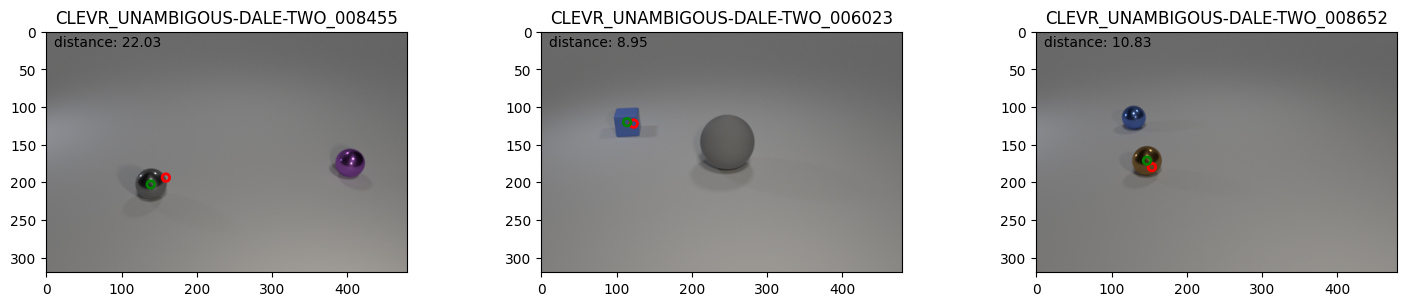
\includegraphics[width=1\linewidth]{figures/visualization_dale-2_train.png}
        \label{fig:visualizations_dale-2_train}
    }
    \subfigure['Dale-2', test split]{
        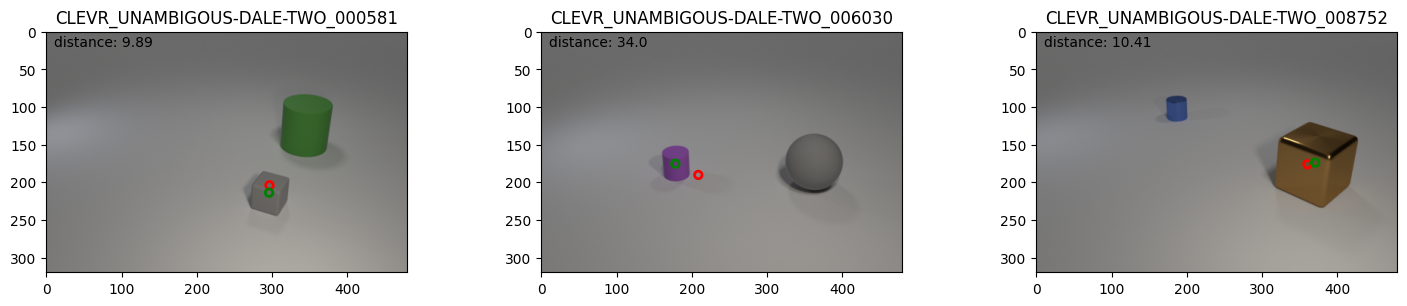
\includegraphics[width=1\linewidth]{figures/visualization_dale-2_test.png}
        \label{fig:visualizations_dale-2_test}
    }
    \subfigure['Dale-5', train split]{
        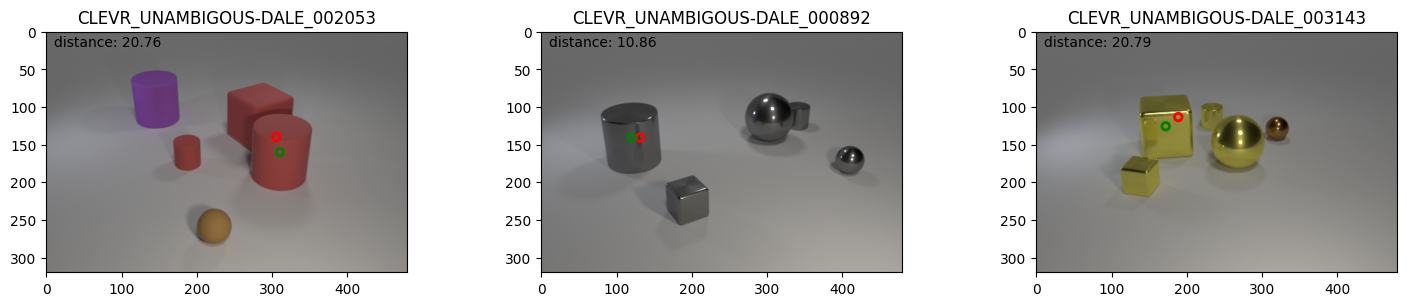
\includegraphics[width=1\linewidth]{figures/visualization_dale-5_train.png}
        \label{fig:visualizations_dale-5_train}
    }
    \subfigure['Dale-5', test split]{
        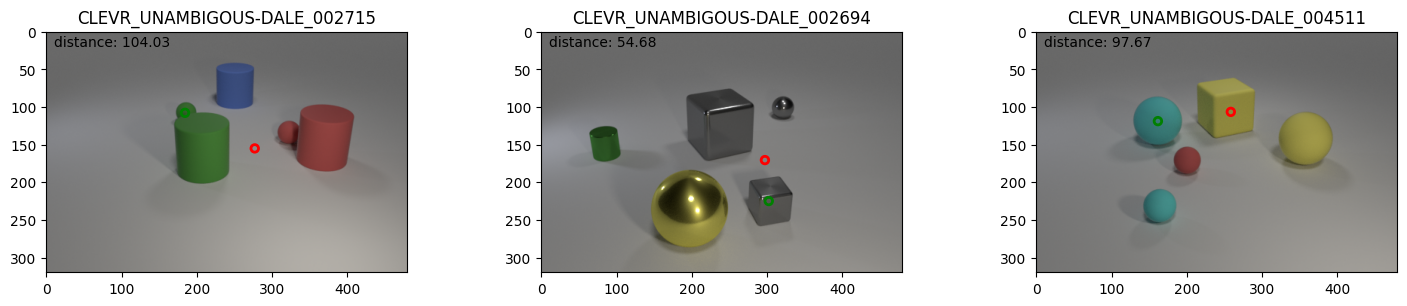
\includegraphics[width=1\linewidth]{figures/visualization_dale-5_test.png}
        \label{fig:visualizations_dale-5_test}
    }
    \caption{Visualization of the models' predictions in the 'Dale' datasets}
    \label{fig:visualizations_dale}
\end{figure}

An interesting pattern appears when doing a qualitative analysis of the models' predictions.
Here, I visualized the predicted coordinates compared to the ground truth coordinates.
Figure \ref{fig:visualizations_dale-2_train} shows random examples of predictions for images in the train dataset of Dale-2.
The green circle shows the ground truth center coordinates of the target object, while the red circle shows the prediction of the model.
As can be seen, the prediction are very precise.
Figure \ref{fig:visualizations_dale-2_complete_train} combines the predictions and ground truths across all images in the train dataset.
Here, all predicted coordinates are placed as red circles into the image, while all ground truth coordinates are places as green circles.
The resulting shape is a rhombus, which reflects that all objects are placed usually central into the scene.
As expected the green and red rhombus align mostly in the same area for the train split of the 'Dale-2' dataset.

The results look very different for the test split.
As can be seen in Figure \ref{fig:visualizations_dale-2_test}, the three randomly selected predictions don't align with the ground truth coordinates.
For all the images, the predictions don't lie on any object.
In the left image as well as in the central image, the predictions are closer to the target object than towards the distractor, but are still quite imprecise.
These findings align with the mean distance scores, described in the sections before.
However, it seems that the model's predictions are all towards the center of the image.
This can be seen clearer in Figure \ref{fig:visualizations_dale-2_complete_test}.
Again, the green circles form the shape of rhombus.
In contrast, the predictions in red almost all cluster in the center of the image.
They form roughly the shape of a smaller rhombus.
This behavior can be observed for all datasets and architectures of the model.
Figures \ref{fig:visualizations_dale-5_train}, \ref{fig:visualizations_dale-5_test}, \ref{fig:visualizations_dale-5_complete_train} and \ref{fig:visualizations_dale-5_complete_test} show the results for the 'Dale-5' dataset.
Here, the model more likely predicts the center coordinates of a distractor object as seen in the right image, which is also reflected in the lower score of the mean distance.
Also the combined visualization shows the same clustering of predictions in the center of the scene, but pattern of the smaller rhombus is better visible.

\begin{figure}[h]
    \centering
    \subfigure['Dale-2', train split]{
        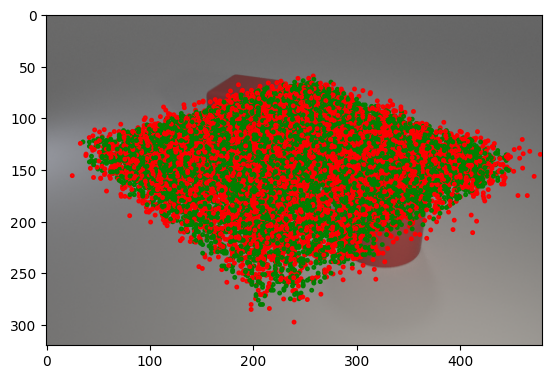
\includegraphics[width=0.42\linewidth]{figures/visualization_dale-2_train_complete.png}
        \label{fig:visualizations_dale-2_complete_train}
    }
    \subfigure['Dale-2', test split]{
        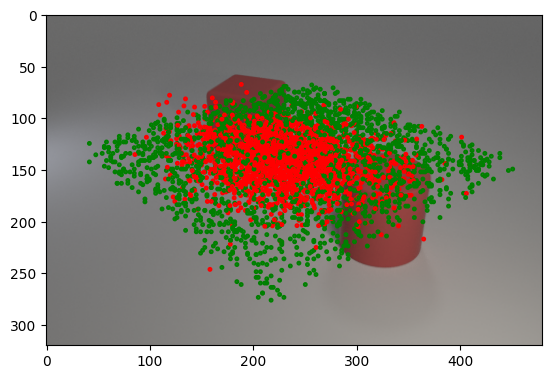
\includegraphics[width=0.42\linewidth]{figures/visualization_dale-2_test_complete.png}
        \label{fig:visualizations_dale-2_complete_test}
    }
    \subfigure['Dale-5', train split]{
        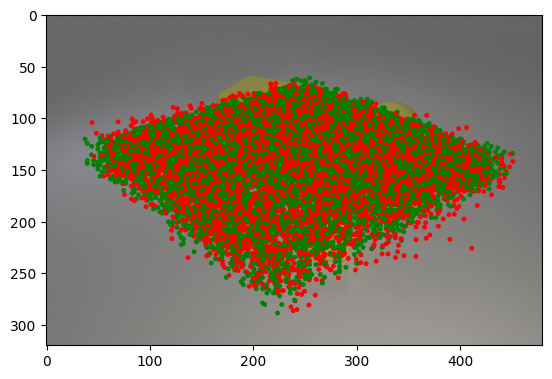
\includegraphics[width=0.42\linewidth]{figures/visualization_dale-5_train_complete.png}
        \label{fig:visualizations_dale-5_complete_train}
    }
    \subfigure['Dale-5', test split]{
        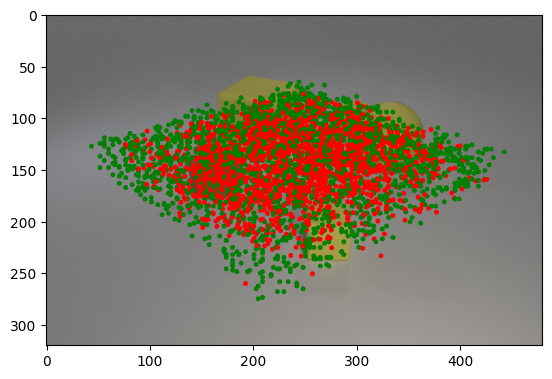
\includegraphics[width=0.42\linewidth]{figures/visualization_dale-5_test_complete.png}
        \label{fig:visualizations_dale-5_complete_test}
    }
    \caption{Visualization of the models' predictions in the Dale datasets}
    \label{fig:visualizations_dale_complete}
\end{figure}

These results allow two conclusions.
First, the models are biased to predict

Second, even though the models are biased towards the center of the image, the predictions are still often leaning in the direction of the target object.
This indicates that it is still able to

\subsubsection{Bounding Box classifier}

\subsubsection{Caption generator}
In the next paragraphs, the results of the caption generator will be discussed.
Table \ref{tab:results_caption-generator} shows the different scores of the models, when trained on 'Dale-2' and 'Dale-5'.
ResNet-3 produced the best results, when it was used as a feature extractor.
The results are shown after 50 epochs, but the scores already start to converge after 20 epochs and changed only very in the following epochs.

\begin{table}[h]
    \centering
    \begin{tabular}{rccc}
        \toprule
                               & \textbf{Accuracy} & \textbf{Word-by-word accuracy} & \textbf{Non-target accuracy} \\
        \textbf{Dale-2}        & 49\%              & 82\%                           & 48\%                         \\
        \textbf{Dale-2 masked} & 72\%              & 90\%                           & 25\%                         \\
        \textbf{Dale-5}        & 21\%              & 45\%                           & 40\%                         \\
        \textbf{Dale-5 masked} & 21\%              & 54\%                           & 45\%                         \\
        \bottomrule
    \end{tabular}
    \caption{Results of the caption generator, based on ResNet-3}
    \label{tab:results_caption-generator}
\end{table}

The sum of the \emph{accuracy} and the \emph{non-target-accuracy} adds to 97\%, when trained on the 'Dale-2' dataset.
This means that the models produce almost always correct descriptions of an object in the image.
Moreover, these descriptions are also efficient in the way that they follow the GRE-algorithm of \citet{Dale1995} and only use necessary discriminative attributes.
Features of both objects are therefore extracted perfectly and related to the vocabulary.
As expected, the model has difficulties to decide, which of both objects is the target object, since no information is passed to the model.
With 48\% of the images describing the target object and 49\% of the images describing the distractor, the model uses a random guess.
This changes, when also the masked image is presented to the model.
Then, the accuracy for the target object is with 72\% well above chance.
Still, the wrong descriptions describe almost every time the distractor object.
This indicates that the problem doesn't lie in extracting features of objects, but only in deciding which object in the image to describe.

When the model is trained on the 'Dale-5' dataset, the results are much worse.
Now, without masking only in 61\% of the images, the model describes any of the objects in the image.
With 21\% of these descriptions being a description of the target object, the model again uses a random guess.
Interestingly, passing the masked image to the model doesn't help it to identify the correct object.
The accuracy stays at the same value.
In contrast, the non-target accuracy is increased by 5\% points.
The model is more likely to identify a wrong object.
Furthermore, the word-by-word accuracy increases from 45\% to 54\%.
This increase is likely due to the fact that the description of the target object often shares some attributes with distractor objects.
For instance an image with a target object being a \emph{small red cube} was identified as a \emph{<pad> <pad> cube} when the model didn't receive the masked image.
After also the masked image was passed to the model, it generated the description \emph{small blue cube}.
This was the correct description of a distractor and because of the overlap of the attributes, the word-by-word accuracy increased from 33\% to 66\%.

The approach, how the padding is produced and in which order the attributes are concatenated didn't have an effect on the described metrics.
When the order was reversed and the padding appended, it seemed like the model was converging slightly faster and reaching the limit around tow to three epochs earlier.
The final peak stayed exactly the same and the effect was therefore not studied deeper if there is an actual significant difference.

There are two main possible explanations for the big difference between the two datasets.
First, as already seen in the experiments before, the bigger number of distractors confuses the model more, where to focus on.
In the 'Dale-2' dataset, there are only two possibilities, while the four distractors in the 'Dale-5' dataset give the model a bigger choice.
The second explanation lies in the used GRE-algorithm.
When only two random objects are placed in a scene, the probability that only the shape is enough to discriminate the objects is at 66,6\%, namely the caption is only one word long.
For shape and color, the probability lies at 29,2\% and that all three attributes are necessary is 4,1\%.
Opposed to that the probabilities with four distractors are 19,8\%, 47\% and 33,2\% respectively.
With four distractors the algorithm is much more likely to produce longer captions.
These are harder to generate for the model, since it needs to take more attributes into account to discriminate the target object from the distractors.

\subsection{Language games}
\subsubsection{Discrimination games}
There are five variables in the experiments that are adjusted:
(1) the image embedding size for the sender $e_s$, (2) the LSTM hidden size for the sender $h_s$, (3) the image/message embedding size for the receiver $e_r$, (4) the LSTM hidden size for the receiver $h_r$ and (5) the size of the vocabulary $|V|$.

Table \ref{tab:results} shows the accuracy of the models calculated on the success of communication if the receiver can identify the target object.
A random guess corresponds to 50\% in the \emph{Dale-2} dataset and 20\% in the \emph{Dale-5} dataset.

\begin{table}[h]
    \centering
    \begin{tabular}{c|ccccc|c}
        \hline
        \textbf{Dataset} & $h_{s}$ & $e_{s}$ & $h_{r}$ & $e_{r}$ & $|V|$ & \textbf{Acc.} \\
        \hline
        Dale-2           & {10}    & {10}    & {10}    & {10}    & {10}  & {95\%}        \\
        Dale-2           & {50}    & {50}    & {128}   & {128}   & {10}  & {50\%}        \\
        Dale-5           & {10}    & {10}    & {10}    & {10}    & {10}  & {23\%}        \\
        Dale-5           & {10}    & {10}    & {10}    & {10}    & {20}  & {23\%}        \\
        Dale-5           & {10}    & {10}    & {10}    & {10}    & {100} & {41\%}        \\
        \hline
    \end{tabular}
    \caption{Results: $h$ are different hidden sizes, $e$ embedding sizes and $|V|$ vocabulary sizes.}
    \label{tab:results}
\end{table}

For the \emph{Dale-2}, a clear correlation between the hidden sizes, embedding sizes and the size of the vocabulary can be identified.
A hidden/embedding size as high as the vocabulary size is beneficial for identifying the correct object.
The receiver identifies almost every sample correctly when all sizes are 10.
When the hidden and embedding sizes are increased, the guesses by the receiver are random with 50\% accuracy.
Interestingly, a vocabulary size of 10 is enough to communicate a meaningful message when the model is trained on the \emph{Dale-2} dataset.

The results change, when using the \emph{Dale-5} dataset with four distractors.
With four distractors and with low hidden, embedding and vocabulary sizes, the agents barely pass the random baseline with 23\%.
Only increasing the vocabulary size to 100 raises the accuracy by almost 20\% points to 43\%.
This is still considerably lower than the 95\% of the \emph{Dale-2} dataset.

\cmtDK{calculation of loss?}

Two conclusions can be drawn.
First, the hidden as well as the embedding sizes need to be close to the vocabulary size.
This even applies for very low vocabulary sizes, which means that the image encodings need to be compressed to the same low dimensions.
The reason for this is very likely that neural models have difficulties to upscale from lower dimensions (e.g. from low $h_r$ to high $e_r$) as opposed to learn how to extract the important information from a vector with many dimensions.

The second conclusion that can be drawn looks at the differences between the two datasets.
Unsurprisingly, the agents have a much higher difficulty to discriminate a target object from four instead of one distractor.
Since we discriminate objects based on properties that are also distinguished in human cognition (color, size, shape), we expect that the vocabulary onto which the agents converge reflects these categories and is therefore close to human vocabulary.
There are 48 possible combinations of attributes.
Still, for Dale-2, a vocabulary size of only 10 is enough for an almost perfect accuracy with two objects.
This hints to the fact that the agents don't describe the complete target object, but only rely on discriminative attributes between the objects.
The need for a more detailed description of discriminative attributes is higher when more distractors are involved.
Therefore, the models need to learn more combinations of symbols in order to attest to this higher level of detail and especially how to relate them to features in the images.

\cmtDK{look at language}
\cmtDK{test different sizes}
\cmtDK{similarity to bounding box classifier}

\subsubsection{Caption generators}

\subsubsection{Coordinate predictors}